\chapter{内核雏形}\label{cha:latex-brief-intro}

\section{实验内容}
进程切换;丰富中断处理程序,比如让时钟中断处理可以不停地发生而不是只发生一次,进程状态的保存与恢复,进程调度,解决中断重入问题。

\section{代码分析}

\subsection{核心数据结构}

\begin{table}[H]
\begin{center}
\caption{主要数据结构}
\begin{tabular}{|c|l|l|}
\hline
\multirow{2}{*}{结构体} & STACK\_FRAME       & 进程表结构体的定义 \\ \cline{2-3} 
                     & PROCESS            & 进程结构体的定义  \\ \hline
\multirow{2}{*}{宏}   & NR\_TASKS          & 最大允许进程:1  \\ \cline{2-3} 
                     & STACK\_SIZE\_TOTAL & 栈的大小      \\ \hline
\end{tabular}
\end{center}
\end{table}


\subsection{关键代码分析}
\begin{enumerate}
    \item \texttt{[section .text]}
    \texttt{global \_start}:让\texttt{\_start}符号成为可见的标识符,这样链接器就知道跳转到程序中的什么地方并开始执行程序。
    \texttt{\_start}:
    设置参数三:字符串长度
    设置参数二:要显示的字符串
    设置参数一:文件描述符(\texttt{stdout})

    \item 系统调用号(\texttt{sys\_write}):调用内核功能进行写操作
    系统调用号(\texttt{sys\_exit}):调用内核功能进行退出操作
    
    \item \texttt{[section .text]}
    外部函数\texttt{extern choose}
    \texttt{\_start}:
    将\texttt{num2nd}和\texttt{num1st}推入栈中
    调用外部函数\texttt{choose}
    增加栈指针8个字节
    系统调用号(\texttt{sys\_exit}):调用内核功能进行退出操作

    \item \texttt{myprint}函数:设置参数二:\texttt{len},设置参数一:\texttt{msg}
    设置参数:文件描述符(\texttt{stdout})
    
    \item 系统调用号(\texttt{sys\_write}):调用内核功能进行写操作

    \item 文件\texttt{bar.c}:
    声明外部函数\texttt{myprint()}
    定义\texttt{choose()}函数
    若\texttt{a >= b}:
    调用\texttt{myprint}输出"the 1st one"
    否则:
    调用\texttt{myprint}输出"the 2nd one"
    
    \item 文件\texttt{loader.asm}
    
    \item 使\texttt{ds}、\texttt{es}、\texttt{ss}三个段寄存器指向与\texttt{cs}相同的段,设置栈指针\texttt{sp}指向栈底

    \item 清屏并显示字符串"Booting"

    \item 软驱复位

    \item 在A盘的根目录中查找\texttt{LOADER.BIN}:遍历根目录,加载每个扇区到内存中,然后从中寻找文件名为\texttt{Loader.bin}的条目,直到找到为止。每读取一个扇区,在"Booting"后面打一个点。在成功加载和执行后显示字符串"Ready"。将控制权正式转移到已加载到内存中的\texttt{LOADER.BIN}的开头,开始执行其代码。

    \item \texttt{DispStr}函数:显示一个字符串

    \item \texttt{ReadSector}函数:从第\texttt{ax}个扇区开始,将\texttt{cl}个扇区读入\texttt{es:bx}中

    \item \texttt{GetFATEntry}函数:在FAT中找到序号为\texttt{ax}的扇区的条目,结果存储在\texttt{ax}中。需要注意的是,在过程中需要将FAT扇区读入\texttt{es:bx},因此函数开始时保存了\texttt{es}和\texttt{bx}。

    \item \texttt{KillMotor}函数:关闭软驱马达
    
    \item 文件\texttt{Kernel.asm}:
    \texttt{[section .text]}
    \texttt{global \_start};导出\texttt{\_start}
    跳转到\texttt{\_start},假设\texttt{gs}指向视频内存。设置黑底白字。设置\texttt{AL='K'}。在\texttt{gs}的偏移位置(屏幕第1行39列)写入字符'L'。
    无限循环。
    
    \item 文件\texttt{loader.asm}:
    重新整理和对齐\texttt{KERNEL.BIN}的内容,将其放置在一个新位置。迭代每个程序头,根据程序头中的信息确定将什么内容放入内存中,放在何处,以及放置多少。
\end{enumerate}


\section{调试过程及结果分析}
调试时主要出现以下问题,运行链接指令:ld -s hello.o -o hello报错,查阅资料后得知该指令只适用于 32 位操作系统的环境,而我们现在使用的操作系统为 64 位。因此修改为:ld -m elf$\_$i386 -o hello hello.o,修改后成功运行,结果如下图6-1所示:
\begin{figure}[H]
  \centering
  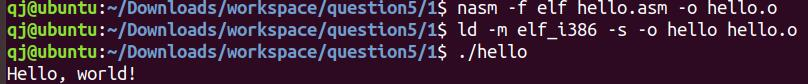
\includegraphics[width=0.8\textwidth]{figures/chapter6/6-1.jpg}
  \caption{汇编语言 Hello World 运行结果 }
  \label{fig:1}
\end{figure}

同样地,在编译时也需要指定32位的方式,使用以下指令:gcc -m32 -c -o bar.o bar.c。foobar运行结果如下图6-2所示:
\begin{figure}[H]
  \centering
  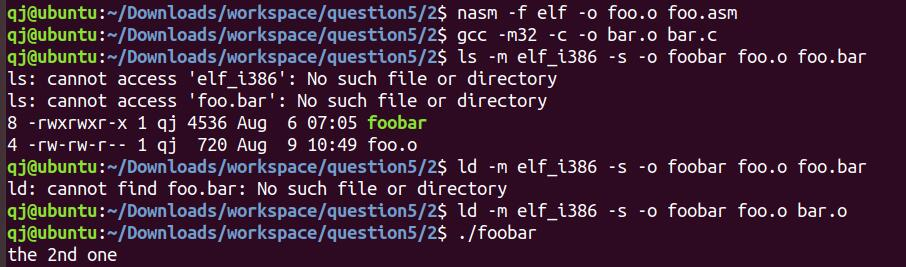
\includegraphics[width=0.8\textwidth]{figures/chapter6/6-2.jpg}
  \caption{foobar 执行结果}
  \label{fig:2}
\end{figure}

在此处,定义了 num1=3,num2=4,程序输出大的那个数的结果,可以看到,程序输出了“the 2nd one”的字样,成功完成了任务。接着,我们以同样方式编译boot,loader和kernel,调试运行结果如下图6-3所示:
\begin{figure}[H]
  \centering
  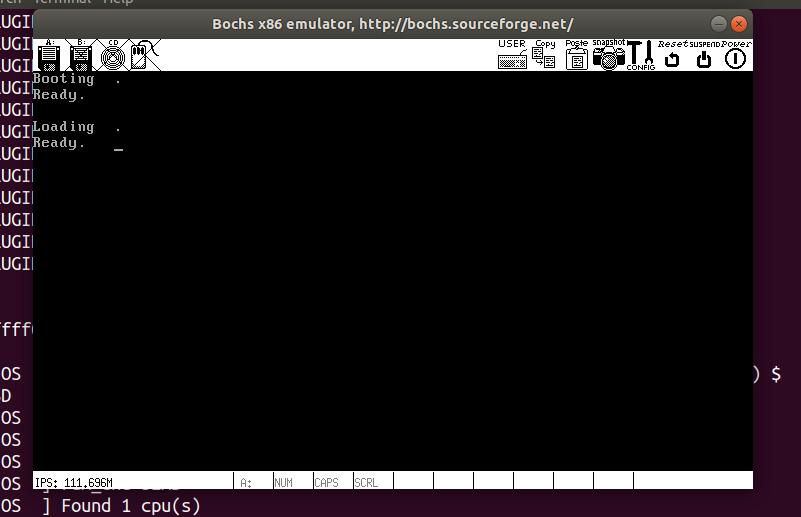
\includegraphics[width=0.8\textwidth]{figures/chapter6/6-3.jpg}
  \caption{载入内核}
  \label{fig:3}
\end{figure}

可以看到,在上一个实验的基础上,这次的实验结果多出了“Loading……”及“Ready.”这样的两行,说明我们已经载入了内核,并且由 Loader 读取了扇区。此外,还要将控制权交给内核,并重新进行调试,结果如下图6-4所示:
\begin{figure}[H]
  \centering
  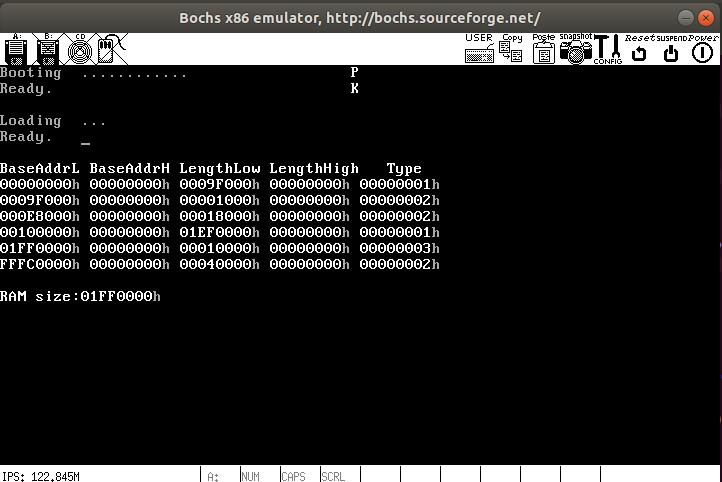
\includegraphics[width=0.8\textwidth]{figures/chapter6/6-4.jpg}
  \caption{控制权交给内核}
  \label{fig:4}
\end{figure}

\section{实验总结}
在本实验中,我们的程序定义了两个节(Section),一个放数据,一个放代码。在代码中值得注意的一点是,入口点默认的是“$\_$start”,在定义它之后还要通过 global 这个关键字让连接程序找到它。代码本身则利用了两个系统调用。\par
实验要结合本机的环境进行,书上使用的是 32 位虚拟机,而现在的Ubuntu更多地是 64 位环境,因此需要针对这一点进行更改。\par
另一方面 ,本章节所实现的操作系统内核已经达到可以使用高级语言程序的地步了,这使得我们后面增加新功能的时候更加方便,可以更多地使用我们更习惯的c语言而不需要再去写底层的汇编语言。除此之外我们也为后面使用 Makefile 文件做好了铺垫,以便我们可以免去那些繁杂重复的工作。这个章节操作和实现上均较简单,但是是意义重大的承上启下的一步——我们将进入保护模式的复杂操作交给了内核,以后这些重复性工作将由内核替我们完成。\par


